
%\special{dvipdfmx:config z 0} %取消PDF压缩,加快速度,最终版本生成的时候最好把这句话注释掉

\documentclass[11pt,a4paper,UTF8]{book}

\usepackage{verbatim}
\usepackage[T1]{fontenc}
\usepackage[utf8]{inputenc}
\usepackage{authblk}

\usepackage{fontspec}                  %引入字体设置宏包
\setmainfont{Times New Roman}             %设置英文正文字体
% Courier New
% Book Antique
\setsansfont{Arial}                    %英文无衬线字体
\setmonofont{Courier New}              %英文等宽字体

\usepackage{ctex} %导入中文包
%\usepackage{ulem}
\usepackage{tocvsec2}


\usepackage{tabularx}
\usepackage{longtable}
\usepackage{booktabs}
\usepackage{multirow}
\usepackage{bbding}
\usepackage{float}
\usepackage{xspace}
\usepackage[none]{hyphenat}
\usepackage{pgffor}

\usepackage{graphicx}
\usepackage{subfigure}
\usepackage{pifont}

\usepackage{hyperref}  %制作pdf的目录
\usepackage{subfiles} %使用多文件方式进行

\usepackage{geometry} %设置页边距的包
\geometry{left=2.5cm,right=2cm,top=2.54cm,bottom=2.54cm} %设置书籍的页边距

\usepackage{url}
\hypersetup{hidelinks, %去红框
  colorlinks=true,
  allcolors=black,
  pdfstartview=Fit,
  breaklinks=true
}

% 调整itemlist中的行间距
\usepackage{enumitem}
\setenumerate[1]{itemsep=0pt,partopsep=0pt,parsep=\parskip,topsep=5pt}
\setitemize[1]{itemsep=0pt,partopsep=0pt,parsep=\parskip,topsep=5pt}
\setdescription{itemsep=0pt,partopsep=0pt,parsep=\parskip,topsep=5pt}

% 超链接样式设置
\usepackage{hyperref}
\hypersetup{
  colorlinks=true,
  linkcolor=blue,
  filecolor=blue,
  urlcolor=blue,
  citecolor=cyan,
}

\usepackage{indentfirst}

\usepackage{listings}
\usepackage[usenames,dvipsnames,svgnames, x11names]{xcolor}
\usepackage{wallpaper}

\usepackage[most]{tcolorbox}
\tcbuselibrary{breakable, minted, skins}

%https://tex.stackexchange.com/questions/173850/problem-in-adding-a-background-color-in-a-minted-environment
\newtcblisting{shell}{
    listing engine=minted,
    minted language=text,%bash, % 使用text就不会有语法高亮显示
    minted options={autogobble,linenos,breaklines},
    listing only,
    size=title,
    arc=0.3mm,
    breakable,
    enhanced jigsaw,
    colframe=black!50!white,
    boxrule=0.5mm,
    colback=bashcodebg,
    coltext=Black,
    minted options={linenos=false,texcl=true},
}
\definecolor{bashcodebg}{rgb}{0.85,0.85,0.85}

% https://tex.stackexchange.com/questions/304449/combine-minted-and-tcolorbox-for-code-from-file-inputminted
\newcounter{inputPrg}
\newtcblisting[use counter=inputPrg, number format=\arabic]{cpp}{
    listing engine=minted,
    minted language=c++,
    minted options={autogobble,linenos,breaklines},
    listing only,
    size=title,
    arc=0.5mm,
    breakable,
    enhanced jigsaw,
    colframe=black!7!white,
    %coltitle=White,
    boxrule=0.5mm,
    colback=blue!3!white,
    coltext=Black,
    %title=\TwoSymbolsAndText{\faCode}{%
        %    \textbf{Input program \thetcbcounter}\ifthenelse{\equal{#2}{}}{}{\textbf{:} \textit{#2}}%
        %}{\faCode},
    %label=inputPrg:#3
    left=6.5mm,enhanced,
    overlay={\begin{tcbclipinterior}\fill[black!5] (frame.south west)
            rectangle ([xshift=5mm]frame.north west);\end{tcbclipinterior}}
}

\usepackage{tikz}

% URL 正确换行
% https://liam.page/2017/05/17/help-the-url-command-from-hyperref-to-break-at-line-wrapping-point/
\makeatletter
\def\UrlAlphabet{%
  \do\a\do\b\do\c\do\d\do\e\do\f\do\g\do\h\do\i\do\j%
  \do\k\do\l\do\m\do\n\do\o\do\p\do\q\do\r\do\s\do\t%
  \do\u\do\v\do\w\do\x\do\y\do\z\do\A\do\B\do\C\do\D%
  \do\E\do\F\do\G\do\H\do\I\do\J\do\K\do\L\do\M\do\N%
  \do\O\do\P\do\Q\do\R\do\S\do\T\do\U\do\V\do\W\do\X%
  \do\Y\do\Z}
\def\UrlDigits{\do\1\do\2\do\3\do\4\do\5\do\6\do\7\do\8\do\9\do\0}
\g@addto@macro{\UrlBreaks}{\UrlOrds}
\g@addto@macro{\UrlBreaks}{\UrlAlphabet}
\g@addto@macro{\UrlBreaks}{\UrlDigits}
\makeatother

% enable subsubsubsection
% from https://tex.stackexchange.com/练习题/274212/correct-hierarchy-levels-of-pdf-bookmarks-for-custom-section-subsubsubsection
\usepackage[depth=3]{bookmark}
\setcounter{secnumdepth}{3}
\setcounter{tocdepth}{4}
\hypersetup{bookmarksdepth=4}

\makeatletter

\newcommand{\toclevel@subsubsubsection}{4}
\newcounter{subsubsubsection}[subsubsection]

\renewcommand{\thesubsubsubsection}{\thesubsubsection.\arabic{subsubsubsection}}

\newcommand{\subsubsubsection}{\@startsection{subsubsubsection}{4}{\z@}%
  {-3.25ex\@plus -1ex \@minus -.2ex}%
  {1.5ex \@plus .2ex}%
  {\normalfont\normalsize\bf\bfseries}}

\newcommand*{\l@subsubsubsection}{\@dottedtocline{4}{11em}{5em}}

\newcommand{\subsubsubsectionmark}[1]{}
\makeatother


\ExplSyntaxOn

% Setup enumerate, itemize and description
\setenumerate  { nosep }
\setitemize    { nosep }
\setdescription{ nosep }

% Setup minted
\setminted { obeytabs, tabsize=2, breaklines=true, fontsize=\footnotesize}

% Def \filename
\NewDocumentCommand { \filename } { m }
{ \noindent  \hspace*{\fill} \\ \textit { #1 } \vspace*{ -1ex } \nopagebreak[4] }

% Def \mySamllsection
\NewDocumentCommand { \mySamllsection } { m }
{\vspace{ 0.2cm } \noindent \textbf { #1 } \vspace*{ 0.05cm } \nopagebreak[4] }

\NewDocumentCommand { \myGraphic } { mmm }
{
  \begin{center}
    \includegraphics[width={#1}\textwidth]{#2}\\
    {#3}
  \end{center}
}

% Def \inlcpp
\NewDocumentCommand { \inlcpp }   { m }
{ \mintinline { cpp } { #1 } }

% Def cpp environment
%\NewDocumentEnvironment { cpp } { }
%{ \VerbatimEnvironment
%  \begin { minted } [ linenos=true, frame=single ] { cpp } }
%{ \end   { minted } }

% Def cmake environment
\NewDocumentEnvironment { cmake } { }
{ \VerbatimEnvironment
  \begin { minted } [ linenos=true, frame=single ] { cmake } }
{ \end   { minted } }

\NewDocumentEnvironment { myNotic } { m }
{ %\hspace*{\fill} \\
  \begin { tcolorbox } [ breakable,colback = blue!5!white, colframe=blue!55!black ,title={#1}] }
{ \end   { tcolorbox } }

\NewDocumentEnvironment { myTip } { m }
{ %\hspace*{\fill} \\
  \begin { tcolorbox } [ breakable,colback = green!5!white, colframe=green!45!black ,title={#1}] }
{ \end   { tcolorbox } }

\NewDocumentEnvironment { myWarning } { m }
{ %\hspace*{\fill} \\
  \begin { tcolorbox } [ breakable,colback=red!5!white,colframe=red!55!black,title={#1}] }
{ \end   { tcolorbox } }

\NewDocumentCommand { \mySubsubsection } { mm }
{
\subsubsection*{\zihao{3} {#1} \hspace{0.2cm}{#2}}
\addcontentsline{toc}{subsubsection}{{#1}\hspace{0.2cm}{#2}}
}

\NewDocumentCommand { \mySubsectionNoFile } { mm }
{
\subsection*{\zihao{3}{#1}\hspace{0.2cm}{#2}}
\addcontentsline{toc}{subsection}{{#1}\hspace{0.2cm}{#2}}
}

\NewDocumentCommand { \mySubsection } { mmm }
{
\subsection*{\zihao{3}{#1}\hspace{0.2cm}{#2}}
\addcontentsline{toc}{subsection}{{#1}\hspace{0.2cm}{#2}}
\subfile{{#3}}
}

\NewDocumentCommand { \mySectionNoHeadImage } { mmm }
{
\color{black}
\pagecolor{white}
\section*{\zihao{2}{#1}\hspace{0.5cm}{#2}}
\addcontentsline{toc}{section}{{#1}\hspace{0.5cm}{#2}}
\subfile{{#3}}
}

\NewDocumentCommand { \CXXTwentythreeLogo } { mm }
{
\noindent
\begin{picture}(0,0)
\put({#1},{#2}){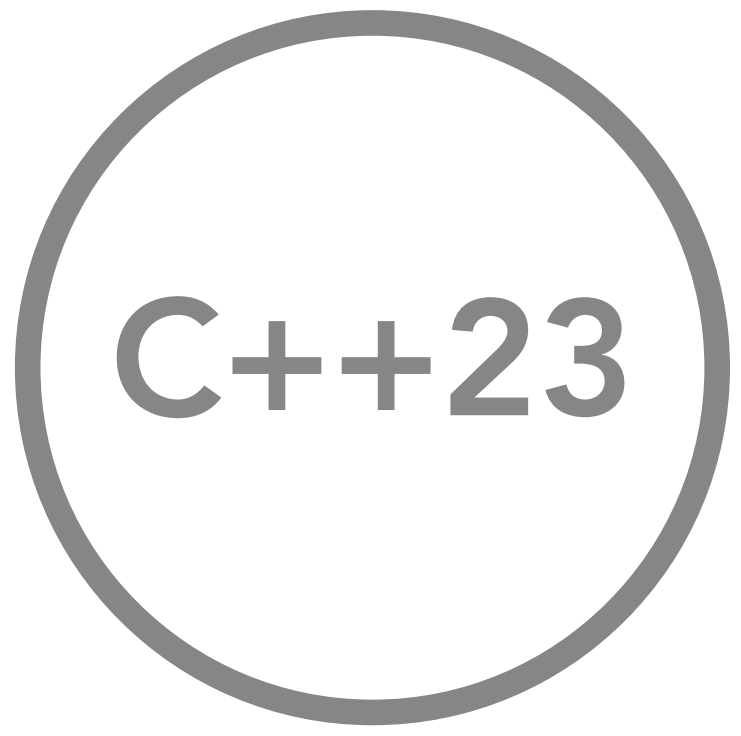
\includegraphics[width=0.07\textwidth]{images/C++23-sign.png}}
\end{picture}
}

\NewDocumentCommand { \mySection } { mmm }
{
\ThisULCornerWallPaper{1.0}{images/section-header.png}
\section*{\zihao{2}{#1}\hspace{0.5cm}{#2}}
\addcontentsline{toc}{section}{{#1}\hspace{0.5cm}{#2}}
\subfile{{#3}}
}

\NewDocumentCommand { \myPart } { mmm }
{
\ThisCenterWallPaper{1.15}{images/section-background.png}
\section*{\zihao{2}{#1}\hspace{0.5cm}{#2}}
\addcontentsline{toc}{section}{{#1}\hspace{0.5cm}{#2}}
\subfile{{#3}}
}

% Latex如何在文本模式批量处理下划线
% https://zhuanlan.zhihu.com/p/615108006

\ExplSyntaxOff

\begin{document}
\begin{sloppypar} %latex中一行文字出现溢出问题的解决方法
%\maketitle

\begin{center}
\thispagestyle{empty}
%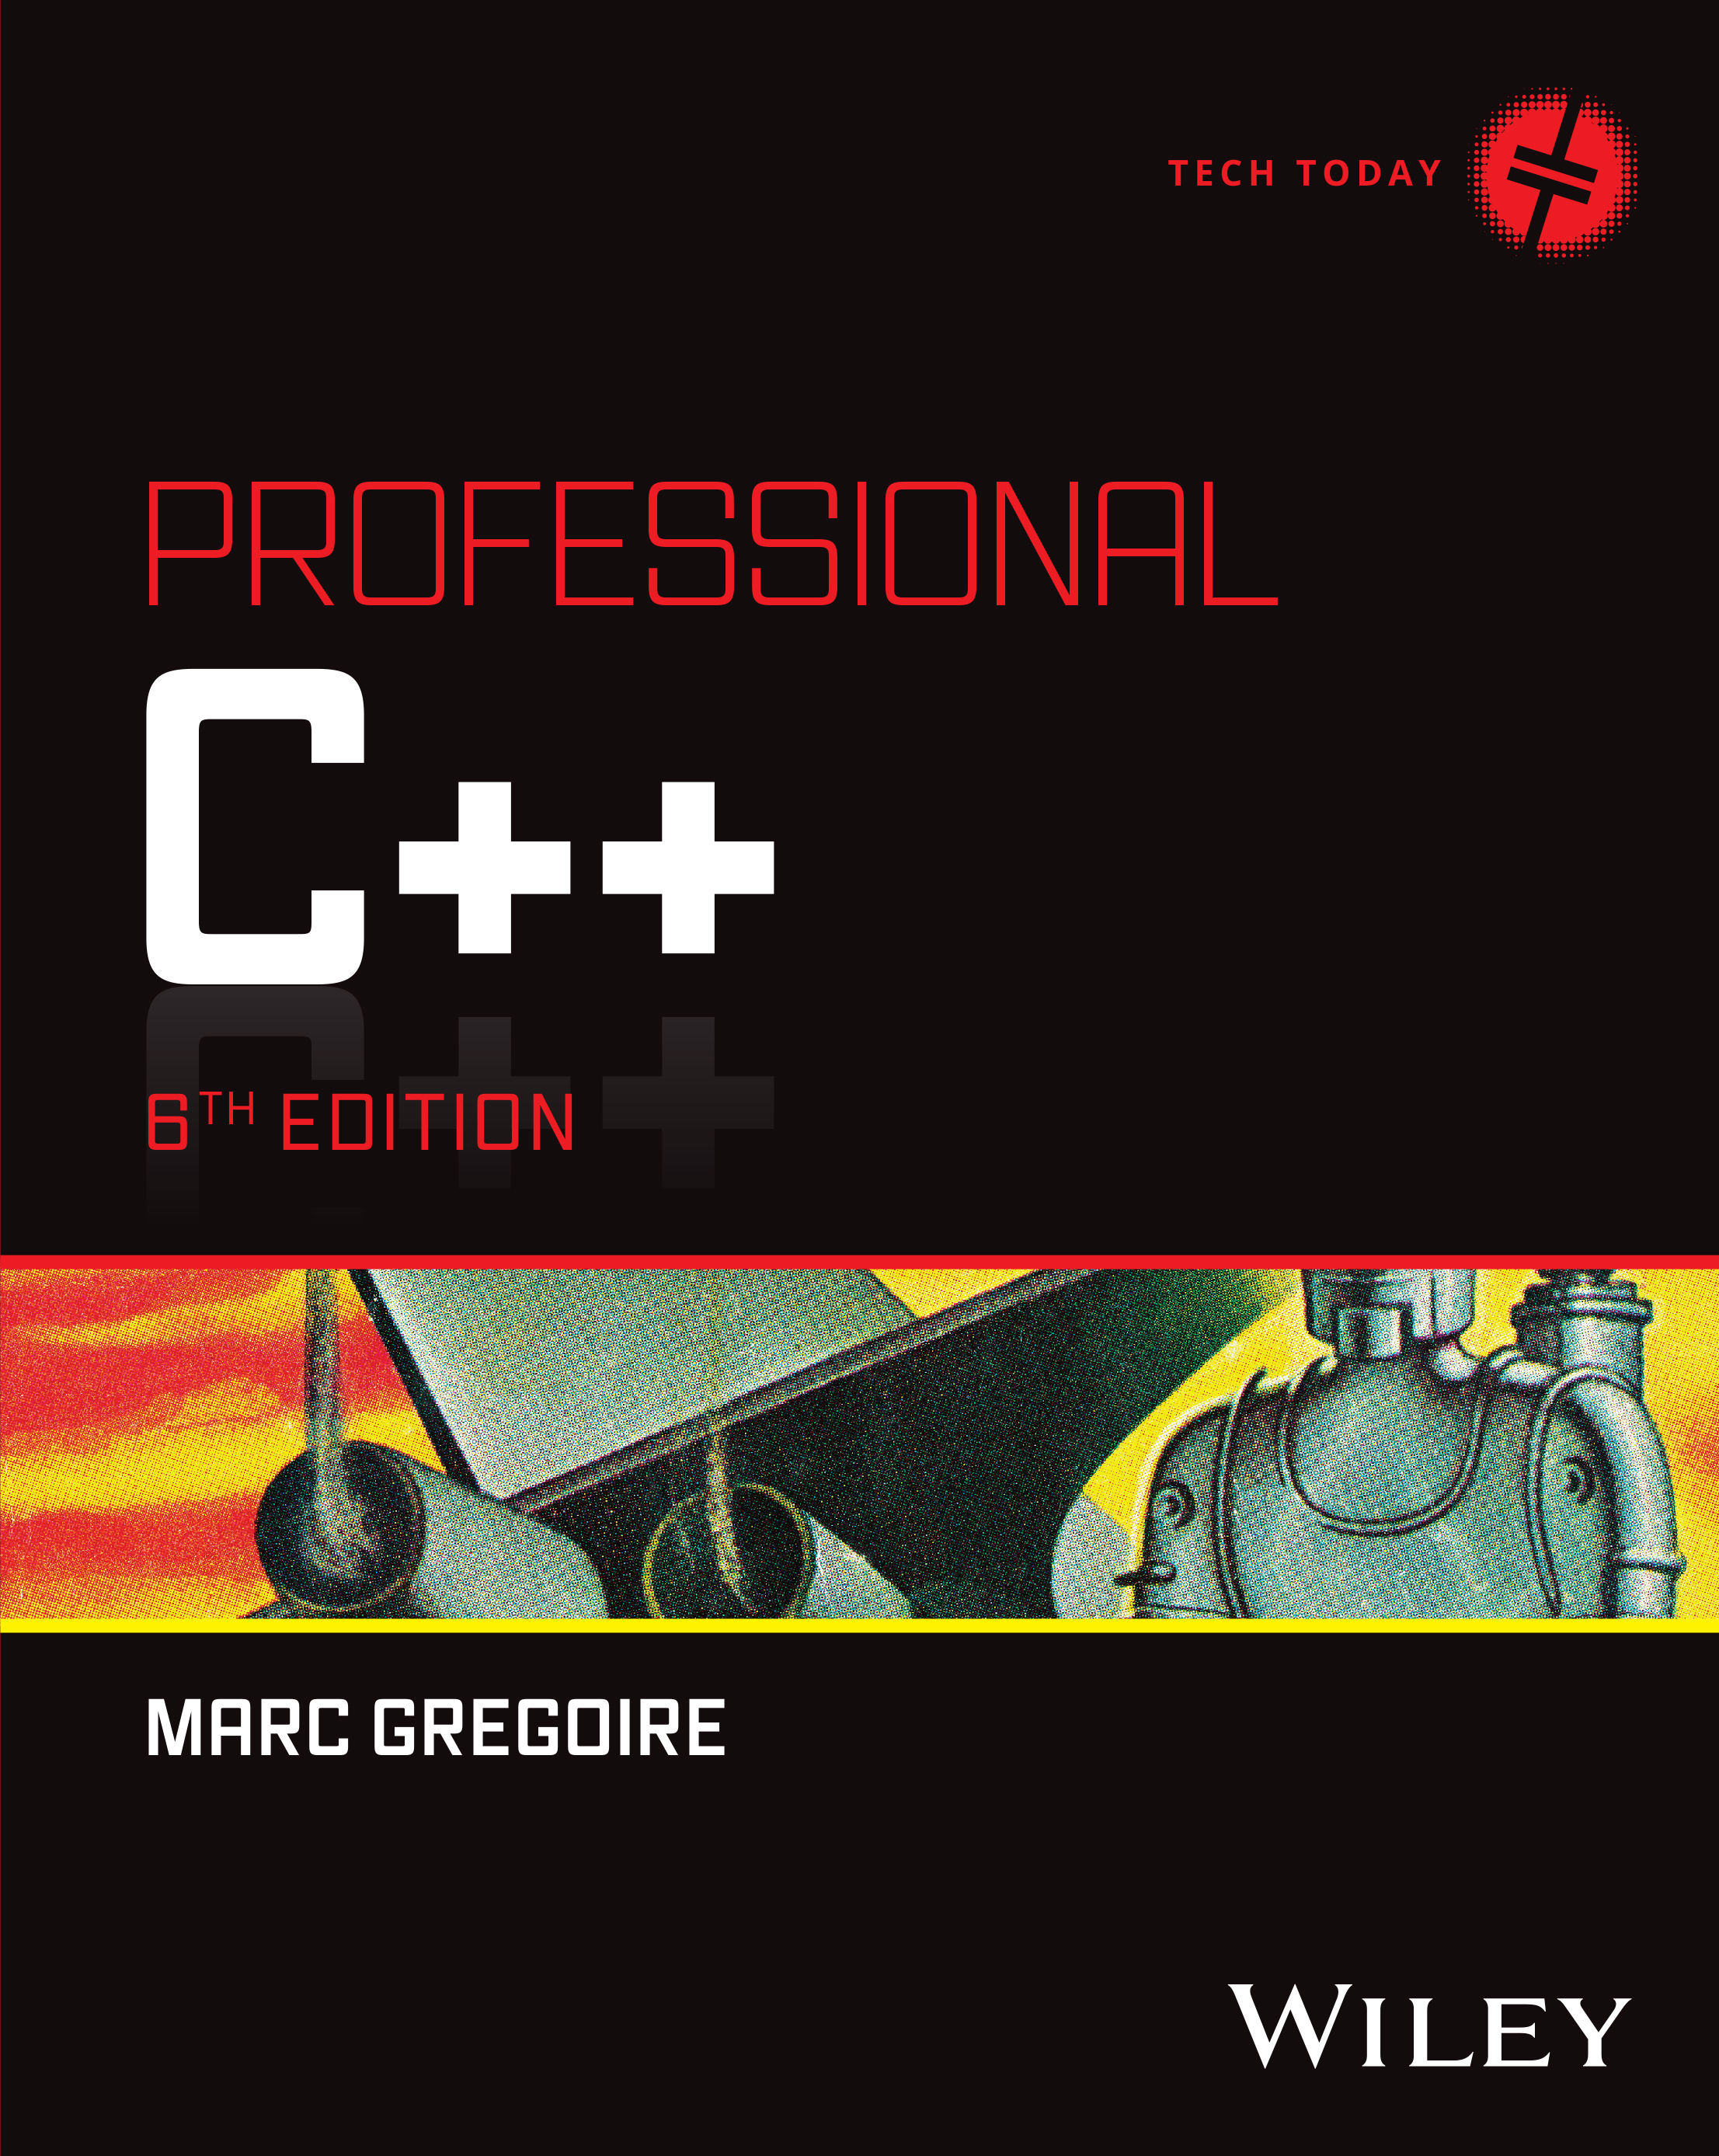
\includegraphics[width=\textwidth,height=\textheight,keepaspectratio]{cover.png}
\begin{tikzpicture}[remember picture, overlay, inner sep=0pt]
\node at (current page.center)
{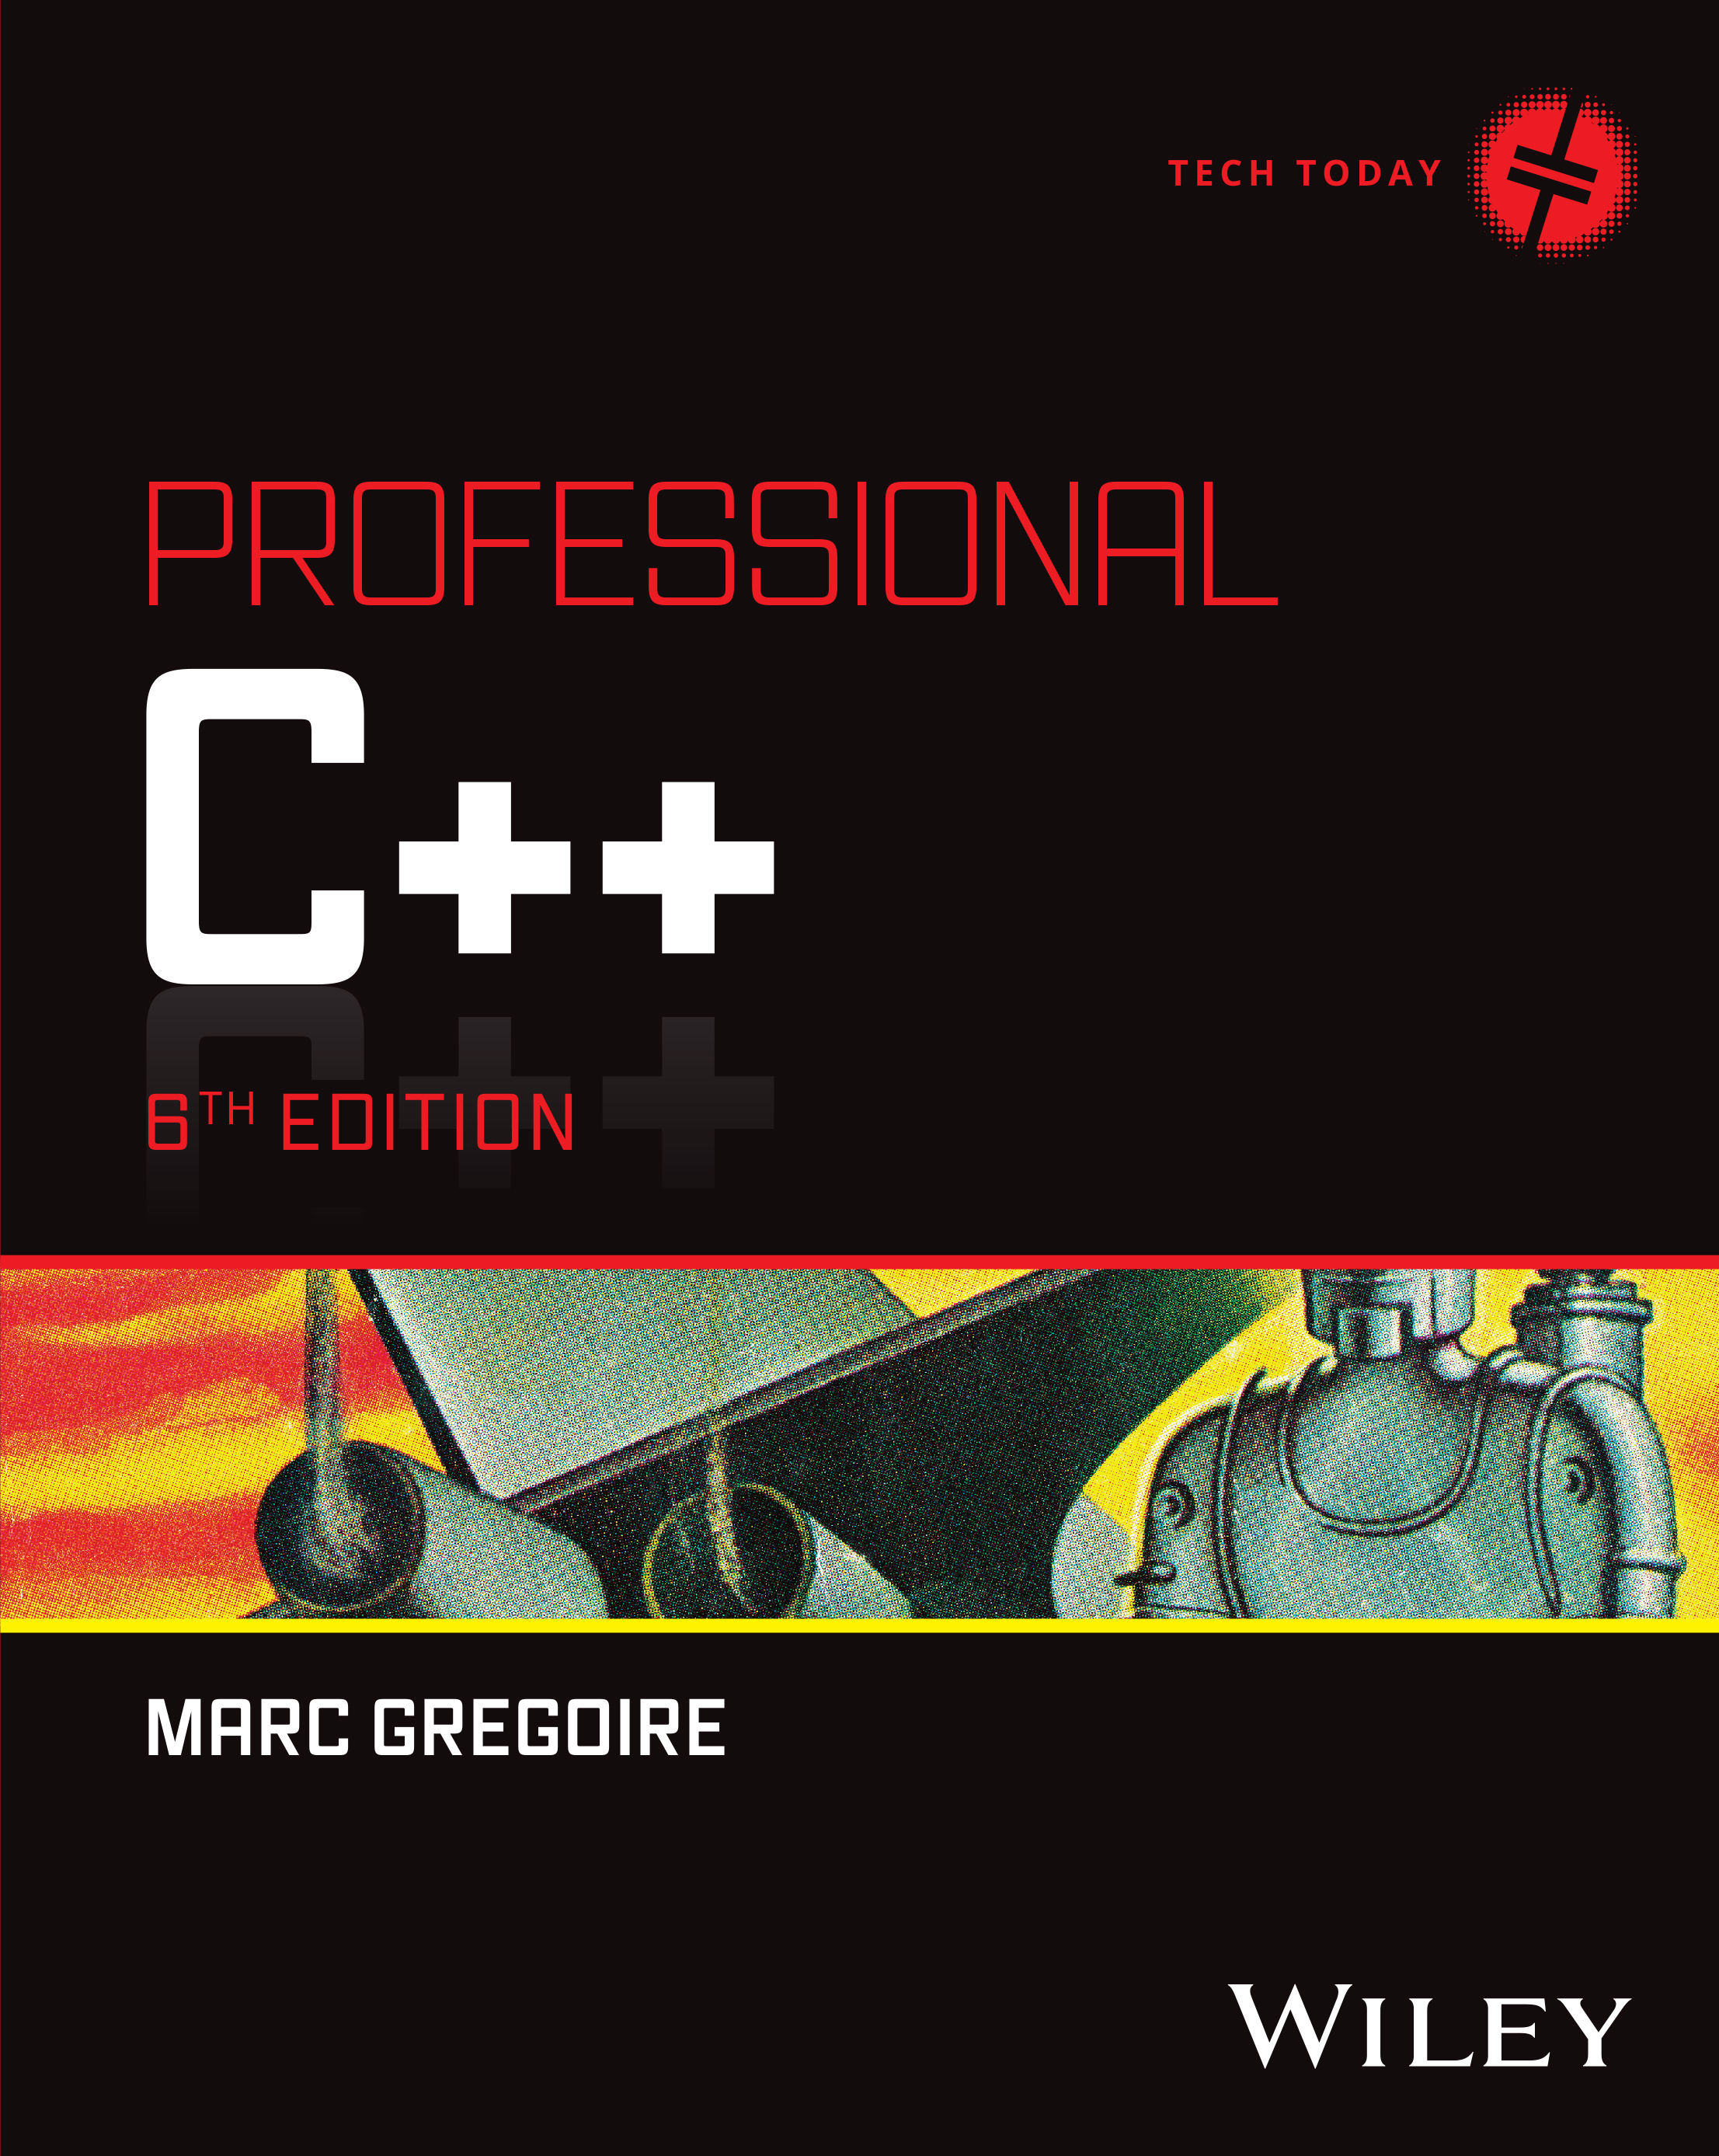
\includegraphics[width=\paperwidth, keepaspectratio=false]{cover.png}};
\end{tikzpicture}
\newpage
\thispagestyle{empty}
\huge
\textbf{Professional C++}
\\[9pt]
{\Large 6th Edition}
\\[9pt]
\normalsize
作者: Marc Gregoire
\\[8pt]
\normalsize
译者:\href{https://github.com/xiaoweiChen/Professional-cpp-6ed}{陈晓伟}
\\[8pt]
\end{center}

\newpage

\begin{comment}
\end{comment}
\pagestyle{empty}
\tableofcontents
\newpage

\setsecnumdepth{section}

\mySectionNoHeadImage{}{关于作者}{content/about-the-author.tex}
\newpage

\mySectionNoHeadImage{}{关于编辑}{content/about-the-technical-editor.tex}
\newpage

\mySectionNoHeadImage{}{致谢}{content/acknowledgment.tex}
\newpage

\mySectionNoHeadImage{}{前言}{content/preface.tex}
\newpage

\myPart{第一部分}{介绍C++}{content/part1.tex}
\newpage

\mySection{第1章}{C++基础知识和标准库}{content/part1/chapter1/0.tex}
\mySubsection{1.1.}{C++基础速成}{content/part1/chapter1/1.tex}
\mySubsection{1.2.}{第一个C++程序}{content/part1/chapter1/2.tex}
\mySubsection{1.3.}{总结}{content/part1/chapter1/3.tex}
\mySubsection{1.4.}{习题}{content/part1/chapter1/4.tex}
\newpage

\mySection{第2章}{字符串和字符串视图}{content/part1/chapter2/0.tex}
\mySubsection{2.1.}{动态字符串}{content/part1/chapter2/1.tex}
\mySubsection{2.2.}{格式化和打印字符串}{content/part1/chapter2/2.tex}
\mySubsection{2.3.}{总结}{content/part1/chapter2/3.tex}
\mySubsection{2.4.}{习题}{content/part1/chapter2/4.tex}
\newpage

\mySection{第3章}{编码风格}{content/part1/chapter3/0.tex}
\mySubsection{3.1.}{代码风格的重要性}{content/part1/chapter3/1.tex}
\mySubsection{3.2.}{编写代码文档}{content/part1/chapter3/2.tex}
\mySubsection{3.3.}{分解}{content/part1/chapter3/3.tex}
\mySubsection{3.4.}{命名}{content/part1/chapter3/4.tex}
\mySubsection{3.5.}{语言特性的风格}{content/part1/chapter3/5.tex}
\mySubsection{3.6.}{格式}{content/part1/chapter3/6.tex}
\mySubsection{3.7.}{风格挑战}{content/part1/chapter3/7.tex}
\mySubsection{3.8.}{总结}{content/part1/chapter3/8.tex}
\mySubsection{3.9.}{习题}{content/part1/chapter3/9.tex}
\newpage

\myPart{第二部分}{专业C++软件设计}{content/part2.tex}
\newpage

\mySection{第4章}{设计专业的C++程序}{content/part2/chapter4/0.tex}
\mySubsection{4.1.}{什么是程序设计?}{content/part2/chapter4/1.tex}
\mySubsection{4.2.}{编程设计的重要性}{content/part2/chapter4/2.tex}
\mySubsection{4.3.}{C++的设计}{content/part2/chapter4/3.tex}
\mySubsection{4.4.}{两条规则}{content/part2/chapter4/4.tex}
\mySubsection{4.5.}{重用现有代码}{content/part2/chapter4/5.tex}
\mySubsection{4.6.}{设计一个国际象棋程序}{content/part2/chapter4/6.tex}
\mySubsection{4.7.}{总结}{content/part2/chapter4/7.tex}
\mySubsection{4.8.}{习题}{content/part2/chapter4/8.tex}
\newpage

\mySection{第5章}{类设计}{content/part2/chapter5/0.tex}
\mySubsection{5.1.}{程序性地思考?}{content/part2/chapter5/1.tex}
\mySubsection{5.2.}{面向对象的思想}{content/part2/chapter5/2.tex}
\mySubsection{5.3.}{类的世界}{content/part2/chapter5/3.tex}
\mySubsection{5.4.}{类内关系}{content/part2/chapter5/4.tex}
\mySubsection{5.5.}{总结}{content/part2/chapter5/5.tex}
\mySubsection{5.6.}{习题}{content/part2/chapter5/6.tex}
\newpage

\mySection{第6章}{为重用而设计}{content/part2/chapter6/0.tex}
\mySubsection{6.1.}{重用思想}{content/part2/chapter6/1.tex}
\mySubsection{6.2.}{如何设计可重用代码}{content/part2/chapter6/2.tex}
\mySubsection{6.3.}{总结}{content/part2/chapter6/3.tex}
\mySubsection{6.4.}{习题}{content/part2/chapter6/4.tex}
\newpage

\myPart{第三部分}{专业C++编程}{content/part3.tex}
\newpage

\mySection{第7章}{内存管理}{content/part3/chapter7/0.tex}
\mySubsection{7.1.}{动态内存}{content/part3/chapter7/1.tex}
\mySubsection{7.2.}{数组指针二象性}{content/part3/chapter7/2.tex}
\mySubsection{7.3.}{底层内存操作}{content/part3/chapter7/3.tex}
\mySubsection{7.4.}{常见的内存陷阱}{content/part3/chapter7/4.tex}
\mySubsection{7.5.}{智能指针}{content/part3/chapter7/5.tex}
\mySubsection{7.6.}{总结}{content/part3/chapter7/6.tex}
\mySubsection{7.7.}{习题}{content/part3/chapter7/7.tex}
\newpage

\mySection{第8章}{类和对象}{content/part3/chapter8/0.tex}
\mySubsection{8.1.}{电子表格示例}{content/part3/chapter8/1.tex}
\mySubsection{8.2.}{类}{content/part3/chapter8/2.tex}
\mySubsection{8.3.}{生命周期}{content/part3/chapter8/3.tex}
\mySubsection{8.4.}{总结}{content/part3/chapter8/4.tex}
\mySubsection{8.5.}{习题}{content/part3/chapter8/5.tex}
\newpage

\mySection{第9章}{类和对象(进阶)}{content/part3/chapter9/0.tex}
\mySubsection{9.1.}{友元}{content/part3/chapter9/1.tex}
\mySubsection{9.2.}{动态分配内存}{content/part3/chapter9/2.tex}
\mySubsection{9.3.}{成员函数}{content/part3/chapter9/3.tex}
\mySubsection{9.4.}{Constexpr和Consteval}{content/part3/chapter9/4.tex}
\mySubsection{9.5.}{数据成员}{content/part3/chapter9/5.tex}
\mySubsection{9.6.}{嵌套类}{content/part3/chapter9/6.tex}
\mySubsection{9.7.}{类内枚举}{content/part3/chapter9/7.tex}
\mySubsection{9.8.}{操作符重载}{content/part3/chapter9/8.tex}
\mySubsection{9.9.}{构建稳定的接口}{content/part3/chapter9/9.tex}
\mySubsection{9.10.}{总结}{content/part3/chapter9/10.tex}
\mySubsection{9.11.}{习题}{content/part3/chapter9/11.tex}
\newpage

\mySection{第10章}{继承技术}{content/part3/chapter10/0.tex}
\mySubsection{10.1.}{构建继承类}{content/part3/chapter10/1.tex}
\mySubsection{10.2.}{复用继承}{content/part3/chapter10/2.tex}
\mySubsection{10.3.}{尊重父类}{content/part3/chapter10/3.tex}
\mySubsection{10.4.}{多态继承}{content/part3/chapter10/4.tex}
\mySubsection{10.5.}{多重继承}{content/part3/chapter10/5.tex}
\mySubsection{10.6.}{有趣且晦涩的继承问题}{content/part3/chapter10/6.tex}
\mySubsection{10.7.}{数据类型转换}{content/part3/chapter10/7.tex}
\mySubsection{10.8.}{总结}{content/part3/chapter10/8.tex}
\mySubsection{10.9.}{习题}{content/part3/chapter10/9.tex}
\newpage

\mySection{第11章}{模块和头文件}{content/part3/chapter11/0.tex}
\mySubsection{11.1.}{模块}{content/part3/chapter11/1.tex}
\mySubsection{11.2.}{预处理指令}{content/part3/chapter11/2.tex}
\mySubsection{11.3.}{链接}{content/part3/chapter11/3.tex}
\mySubsection{11.4.}{头文件}{content/part3/chapter11/4.tex}
\mySubsection{11.5.}{核心语言特性的功能——测试宏}{content/part3/chapter11/5.tex}
\mySubsection{11.6.}{static关键字}{content/part3/chapter11/6.tex}
\mySubsection{11.7.}{C风格的变长参数列表}{content/part3/chapter11/7.tex}
\mySubsection{11.8.}{总结}{content/part3/chapter11/8.tex}
\mySubsection{11.9.}{习题}{content/part3/chapter11/9.tex}
\newpage

\mySection{第12章}{使用模板}{content/part3/chapter12/0.tex}
\mySubsection{12.1.}{模板简介}{content/part3/chapter12/1.tex}
\mySubsection{12.2.}{类模板}{content/part3/chapter12/2.tex}
\mySubsection{12.3.}{函数模板}{content/part3/chapter12/3.tex}
\mySubsection{12.4.}{变量模板}{content/part3/chapter12/4.tex}
\mySubsection{12.5.}{概念}{content/part3/chapter12/5.tex}
\mySubsection{12.6.}{总结}{content/part3/chapter12/6.tex}
\mySubsection{12.7.}{习题}{content/part3/chapter12/7.tex}
\newpage

\mySection{第13章}{C++的I/O}{content/part3/chapter13/0.tex}
\mySubsection{13.1.}{使用流}{content/part3/chapter13/1.tex}
\mySubsection{13.2.}{字符串流}{content/part3/chapter13/2.tex}
\mySubsection{13.3.}{基于Span的流}{content/part3/chapter13/3.tex}
\mySubsection{13.4.}{文件流}{content/part3/chapter13/4.tex}
\mySubsection{13.5.}{双向I/O}{content/part3/chapter13/5.tex}
\mySubsection{13.6.}{文件系统库}{content/part3/chapter13/6.tex}
\mySubsection{13.7.}{总结}{content/part3/chapter13/7.tex}
\mySubsection{13.8.}{习题}{content/part3/chapter13/8.tex}
\newpage

\mySection{第14章}{处理错误}{content/part3/chapter14/0.tex}
\mySubsection{14.1.}{错误和异常}{content/part3/chapter14/1.tex}
\mySubsection{14.2.}{异常机制}{content/part3/chapter14/2.tex}
\mySubsection{14.3.}{异常和多态}{content/part3/chapter14/3.tex}
\mySubsection{14.4.}{重新抛出异常}{content/part3/chapter14/4.tex}
\mySubsection{14.5.}{堆栈展开和清理}{content/part3/chapter14/5.tex}
\mySubsection{14.6.}{源定位}{content/part3/chapter14/6.tex}
\mySubsection{14.7.}{栈跟踪}{content/part3/chapter14/7.tex}
\mySubsection{14.8.}{错误处理}{content/part3/chapter14/8.tex}
\mySubsection{14.9.}{异常安全}{content/part3/chapter14/9.tex}
\mySubsection{14.10.}{总结}{content/part3/chapter14/10.tex}
\mySubsection{14.11.}{习题}{content/part3/chapter14/11.tex}
\newpage

\mySection{第15章}{重载操作符}{content/part3/chapter15/0.tex}
\mySubsection{15.1.}{概述}{content/part3/chapter15/1.tex}
\mySubsection{15.2.}{重载算术操作符}{content/part3/chapter15/2.tex}
\mySubsection{15.3.}{重载位和二进制逻辑操作符}{content/part3/chapter15/3.tex}
\mySubsection{15.4.}{重载插入和提取操作符}{content/part3/chapter15/4.tex}
\mySubsection{15.5.}{重载下标操作符}{content/part3/chapter15/5.tex}
\mySubsection{15.6.}{重载函数调用操作符}{content/part3/chapter15/6.tex}
\mySubsection{15.7.}{重载解引用操作符}{content/part3/chapter15/7.tex}
\mySubsection{15.8.}{写入转换操作符}{content/part3/chapter15/8.tex}
\mySubsection{15.9.}{重载内存分配和释放操作符}{content/part3/chapter15/9.tex}
\mySubsection{15.10.}{重载用户定义的字面量操作符}{content/part3/chapter15/10.tex}
\mySubsection{15.11.}{总结}{content/part3/chapter15/11.tex}
\mySubsection{15.12.}{习题}{content/part3/chapter15/12.tex}
\newpage

\mySection{第16章}{标准库概述}{content/part3/chapter16/0.tex}
\mySubsection{16.1.}{编码原则}{content/part3/chapter16/1.tex}
\mySubsection{16.2.}{C++标准库概述}{content/part3/chapter16/2.tex}
\mySubsection{16.3.}{总结}{content/part3/chapter16/3.tex}
\mySubsection{16.4.}{习题}{content/part3/chapter16/4.tex}
\newpage

\mySection{第17章}{理解迭代器和标准范围库}{content/part3/chapter17/0.tex}
\mySubsection{17.1.}{迭代器}{content/part3/chapter17/1.tex}
\mySubsection{17.2.}{流迭代器}{content/part3/chapter17/2.tex}
\mySubsection{17.3.}{迭代器适配器}{content/part3/chapter17/3.tex}
\mySubsection{17.4.}{范围}{content/part3/chapter17/4.tex}
\mySubsection{17.5.}{总结}{content/part3/chapter17/5.tex}
\mySubsection{17.6.}{习题}{content/part3/chapter17/6.tex}
\newpage

\mySection{第18章}{标准库容器}{content/part3/chapter18/0.tex}
\mySubsection{18.1.}{概述}{content/part3/chapter18/1.tex}
\mySubsection{18.2.}{顺序容器}{content/part3/chapter18/2.tex}
\mySubsection{18.3.}{顺序视图}{content/part3/chapter18/3.tex}
\mySubsection{18.4.}{容器适配器}{content/part3/chapter18/4.tex}
\mySubsection{18.5.}{关联容器}{content/part3/chapter18/5.tex}
\mySubsection{18.6.}{其他容器}{content/part3/chapter18/6.tex}
\mySubsection{18.7.}{总结}{content/part3/chapter18/7.tex}
\mySubsection{18.8.}{习题}{content/part3/chapter18/8.tex}
\newpage

\mySection{第19章}{函数指针,函数对象和Lambda表达式}{content/part3/chapter19/0.tex}
\mySubsection{19.1.}{函数指针}{content/part3/chapter19/1.tex}
\mySubsection{19.2.}{指向成员函数(和数据成员)的指针}{content/part3/chapter19/2.tex}
\mySubsection{19.3.}{函数对象}{content/part3/chapter19/3.tex}
\mySubsection{19.4.}{多态函数包装器}{content/part3/chapter19/4.tex}
\mySubsection{19.5.}{Lambda表达式}{content/part3/chapter19/5.tex}
\mySubsection{19.6.}{调用器}{content/part3/chapter19/6.tex}
\mySubsection{19.7.}{总结}{content/part3/chapter19/7.tex}
\mySubsection{19.8.}{习题}{content/part3/chapter19/8.tex}
\newpage

\mySection{第20章}{标准库算法}{content/part3/chapter20/0.tex}
\mySubsection{20.1.}{算法概述}{content/part3/chapter20/1.tex}
\mySubsection{20.2.}{算法细节}{content/part3/chapter20/2.tex}
\mySubsection{20.3.}{总结}{content/part3/chapter20/3.tex}
\mySubsection{20.4.}{习题}{content/part3/chapter20/4.tex}
\newpage

\mySection{第21章}{字符串本地化和正则表达式}{content/part3/chapter21/0.tex}
\mySubsection{21.1.}{本地化}{content/part3/chapter21/1.tex}
\mySubsection{21.2.}{正则表达式}{content/part3/chapter21/2.tex}
\mySubsection{21.3.}{总结}{content/part3/chapter21/3.tex}
\mySubsection{21.4.}{习题}{content/part3/chapter21/4.tex}
\newpage

\mySection{第22章}{日期和时间}{content/part3/chapter22/0.tex}
\mySubsection{22.1.}{编译时有理数}{content/part3/chapter22/1.tex}
\mySubsection{22.2.}{时间段}{content/part3/chapter22/2.tex}
\mySubsection{22.3.}{时钟}{content/part3/chapter22/3.tex}
\mySubsection{22.4.}{时间点}{content/part3/chapter22/4.tex}
\mySubsection{22.5.}{日期}{content/part3/chapter22/5.tex}
\mySubsection{22.6.}{时区}{content/part3/chapter22/6.tex}
\mySubsection{22.7.}{总结}{content/part3/chapter22/7.tex}
\mySubsection{22.8.}{习题}{content/part3/chapter22/8.tex}
\newpage

\mySection{第23章}{随机数}{content/part3/chapter23/0.tex}
\mySubsection{23.1.}{C风格的随机数生成}{content/part3/chapter23/1.tex}
\mySubsection{23.2.}{随机数引擎}{content/part3/chapter23/2.tex}
\mySubsection{23.3.}{随机数引擎适配器}{content/part3/chapter23/3.tex}
\mySubsection{23.4.}{预定义的引擎和引擎适配器}{content/part3/chapter23/4.tex}
\mySubsection{23.5.}{生成随机数}{content/part3/chapter23/5.tex}
\mySubsection{23.6.}{随机数分布}{content/part3/chapter23/6.tex}
\mySubsection{23.7.}{总结}{content/part3/chapter23/7.tex}
\mySubsection{23.8.}{习题}{content/part3/chapter23/8.tex}
\newpage

\mySection{第24章}{其他标准类型}{content/part3/chapter24/0.tex}
\mySubsection{24.1.}{Variant}{content/part3/chapter24/1.tex}
\mySubsection{24.2.}{Any}{content/part3/chapter24/2.tex}
\mySubsection{24.3.}{Tuple}{content/part3/chapter24/3.tex}
\mySubsection{24.4.}{Optional: 一元操作}{content/part3/chapter24/4.tex}
\mySubsection{24.5.}{Expected}{content/part3/chapter24/5.tex}
\mySubsection{24.6.}{总结}{content/part3/chapter24/6.tex}
\mySubsection{24.7.}{习题}{content/part3/chapter24/7.tex}
\newpage

\myPart{第四部分}{C++高级特性}{content/part4.tex}
\newpage

\mySection{第25章}{自定义和扩展标准库}{content/part4/chapter25/0.tex}
\mySubsection{25.1.}{分配器}{content/part4/chapter25/1.tex}
\mySubsection{25.2.}{扩展标准库}{content/part4/chapter25/2.tex}
\mySubsection{25.3.}{总结}{content/part4/chapter25/3.tex}
\mySubsection{25.4.}{习题}{content/part4/chapter25/4.tex}
\newpage

\mySection{第26章}{模板进阶}{content/part4/chapter26/0.tex}
\mySubsection{26.1.}{模板参数}{content/part4/chapter26/1.tex}
\mySubsection{26.2.}{类模板的偏特化}{content/part4/chapter26/2.tex}
\mySubsection{26.3.}{用重载模拟函的数偏特化}{content/part4/chapter26/3.tex}
\mySubsection{26.4.}{模板递归}{content/part4/chapter26/4.tex}
\mySubsection{26.5.}{变长模板}{content/part4/chapter26/5.tex}
\mySubsection{26.6.}{元编程}{content/part4/chapter26/6.tex}
\mySubsection{26.7.}{总结}{content/part4/chapter26/7.tex}
\mySubsection{26.8.}{习题}{content/part4/chapter26/8.tex}
\newpage

\mySection{第27章}{C++多线程编程}{content/part4/chapter27/0.tex}
\mySubsection{27.1.}{介绍}{content/part4/chapter27/1.tex}
\mySubsection{27.2.}{线程}{content/part4/chapter27/2.tex}
\mySubsection{27.3.}{原子操作库}{content/part4/chapter27/3.tex}
\mySubsection{27.4.}{互斥}{content/part4/chapter27/4.tex}
\mySubsection{27.5.}{条件变量}{content/part4/chapter27/5.tex}
\mySubsection{27.6.}{门闩}{content/part4/chapter27/6.tex}
\mySubsection{27.7.}{栅栏}{content/part4/chapter27/7.tex}
\mySubsection{27.8.}{信号量}{content/part4/chapter27/8.tex}
\mySubsection{27.9.}{Future}{content/part4/chapter27/9.tex}
\mySubsection{27.10.}{示例: 多线程记录器类}{content/part4/chapter27/10.tex}
\mySubsection{27.11.}{线程池}{content/part4/chapter27/11.tex}
\mySubsection{27.12.}{协程}{content/part4/chapter27/12.tex}
\mySubsection{27.13.}{线程设计和最佳实践}{content/part4/chapter27/13.tex}
\mySubsection{27.14.}{总结}{content/part4/chapter27/14.tex}
\mySubsection{27.15.}{习题}{content/part4/chapter27/15.tex}
\newpage

\myPart{第五部分}{C++软件工程}{content/part5.tex}
\newpage

\mySection{第28章}{最大化软件工程方法}{content/part5/chapter28/0.tex}
\mySubsection{28.1.}{过程的必要性}{content/part5/chapter28/1.tex}
\mySubsection{28.2.}{软件生命周期模型}{content/part5/chapter28/2.tex}
\mySubsection{28.3.}{软件工程方法论}{content/part5/chapter28/3.tex}
\mySubsection{28.4.}{建立自己的过程和方法}{content/part5/chapter28/4.tex}
\mySubsection{28.5.}{版本控制}{content/part5/chapter28/5.tex}
\mySubsection{28.6.}{总结}{content/part5/chapter28/6.tex}
\mySubsection{28.7.}{习题}{content/part5/chapter28/7.tex}
\newpage

\mySection{第29章}{编写高效的C++}{content/part5/chapter29/0.tex}
\mySubsection{29.1.}{性能和效率概述}{content/part5/chapter29/1.tex}
\mySubsection{29.2.}{语言级效率}{content/part5/chapter29/2.tex}
\mySubsection{29.3.}{设计级效率}{content/part5/chapter29/3.tex}
\mySubsection{29.4.}{效率分析}{content/part5/chapter29/4.tex}
\mySubsection{29.5.}{总结}{content/part5/chapter29/5.tex}
\mySubsection{29.6.}{习题}{content/part5/chapter29/6.tex}
\newpage

\mySection{第30章}{熟悉测试}{content/part5/chapter30/0.tex}
\mySubsection{30.1.}{质量控制}{content/part5/chapter30/1.tex}
\mySubsection{30.2.}{单元测试}{content/part5/chapter30/2.tex}
\mySubsection{30.3.}{模糊测试}{content/part5/chapter30/3.tex}
\mySubsection{30.4.}{高阶测试}{content/part5/chapter30/4.tex}
\mySubsection{30.5.}{成功测试的技巧}{content/part5/chapter30/5.tex}
\mySubsection{30.6.}{总结}{content/part5/chapter30/6.tex}
\mySubsection{30.7.}{习题}{content/part5/chapter30/7.tex}
\newpage

\mySection{第31章}{征服调试}{content/part5/chapter31/0.tex}
\mySubsection{31.1.}{调试的基本规律}{content/part5/chapter31/1.tex}
\mySubsection{31.2.}{缺陷分类}{content/part5/chapter31/2.tex}
\mySubsection{31.3.}{避免bug}{content/part5/chapter31/3.tex}
\mySubsection{31.4.}{针对bug的计划}{content/part5/chapter31/4.tex}
\mySubsection{31.5.}{调试技术}{content/part5/chapter31/5.tex}
\mySubsection{31.6.}{总结}{content/part5/chapter31/6.tex}
\mySubsection{31.7.}{习题}{content/part5/chapter31/7.tex}
\newpage

\mySection{第32章}{设计技术和框架结合}{content/part5/chapter32/0.tex}
\mySubsection{32.1.}{总是记不住语法怎么办}{content/part5/chapter32/1.tex}
\mySubsection{32.2.}{一定有更好的办法}{content/part5/chapter32/2.tex}
\mySubsection{32.3.}{面向对象框架}{content/part5/chapter32/3.tex}
\mySubsection{32.4.}{总结}{content/part5/chapter32/4.tex}
\mySubsection{32.5.}{习题}{content/part5/chapter32/5.tex}
\newpage

\mySection{第33章}{应用设计模式}{content/part5/chapter33/0.tex}
\mySubsection{33.1.}{策略模式}{content/part5/chapter33/1.tex}
\mySubsection{33.2.}{抽象工厂模式}{content/part5/chapter33/2.tex}
\mySubsection{33.3.}{工厂方法模式}{content/part5/chapter33/3.tex}
\mySubsection{33.4.}{其他工厂模式}{content/part5/chapter33/4.tex}
\mySubsection{33.5.}{适配器模式}{content/part5/chapter33/5.tex}
\mySubsection{33.6.}{代理模式}{content/part5/chapter33/6.tex}
\mySubsection{33.7.}{迭代器模式}{content/part5/chapter33/7.tex}
\mySubsection{33.8.}{观察者模式}{content/part5/chapter33/8.tex}
\mySubsection{33.9.}{装饰器模式}{content/part5/chapter33/9.tex}
\mySubsection{33.10.}{责任链模式}{content/part5/chapter33/10.tex}
\mySubsection{33.11.}{单例模式}{content/part5/chapter33/11.tex}
\mySubsection{33.12.}{总结}{content/part5/chapter33/12.tex}
\mySubsection{33.13.}{习题}{content/part5/chapter33/13.tex}
\newpage

\mySection{第34章}{开发跨平台和跨语言应用程序}{content/part5/chapter34/0.tex}
\mySubsection{34.1.}{跨平台开发}{content/part5/chapter34/1.tex}
\mySubsection{34.2.}{跨语言开发}{content/part5/chapter34/2.tex}
\mySubsection{34.3.}{总结}{content/part5/chapter34/3.tex}
\mySubsection{34.4.}{习题}{content/part5/chapter34/4.tex}
\newpage

\myPart{第六部分}{附录}{content/part6.tex}
\newpage

\mySection{附录A}{C++面试}{content/part6/appendix-A/0.tex}
\mySubsection{A.1.}{第1章}{content/part6/appendix-A/1.tex}
\mySubsection{A.2.}{第2章和第21章}{content/part6/appendix-A/2.tex}
\mySubsection{A.3.}{第3章}{content/part6/appendix-A/3.tex}
\mySubsection{A.4.}{第4章}{content/part6/appendix-A/4.tex}
\mySubsection{A.5.}{第5章}{content/part6/appendix-A/5.tex}
\mySubsection{A.6.}{第6章}{content/part6/appendix-A/6.tex}
\mySubsection{A.7.}{第7章}{content/part6/appendix-A/7.tex}
\mySubsection{A.8.}{第8章和第9章}{content/part6/appendix-A/8.tex}
\mySubsection{A.9.}{第10章}{content/part6/appendix-A/9.tex}
\mySubsection{A.10.}{第11章}{content/part6/appendix-A/10.tex}
\mySubsection{A.11.}{第12章和第26章}{content/part6/appendix-A/11.tex}
\mySubsection{A.12.}{第13章}{content/part6/appendix-A/12.tex}
\mySubsection{A.13.}{第14章}{content/part6/appendix-A/13.tex}
\mySubsection{A.14.}{第15章}{content/part6/appendix-A/14.tex}
\mySubsection{A.15.}{第16-20章和第25章}{content/part6/appendix-A/15.tex}
\mySubsection{A.16.}{第22章}{content/part6/appendix-A/16.tex}
\mySubsection{A.17.}{第23章}{content/part6/appendix-A/17.tex}
\mySubsection{A.18.}{第24章}{content/part6/appendix-A/18.tex}
\mySubsection{A.19.}{第27章}{content/part6/appendix-A/19.tex}
\mySubsection{A.20.}{第28章}{content/part6/appendix-A/20.tex}
\mySubsection{A.21.}{第29章}{content/part6/appendix-A/21.tex}
\mySubsection{A.22.}{第30章}{content/part6/appendix-A/22.tex}
\mySubsection{A.23.}{第31章}{content/part6/appendix-A/23.tex}
\mySubsection{A.24.}{第32章}{content/part6/appendix-A/24.tex}
\mySubsection{A.25.}{第33章}{content/part6/appendix-A/25.tex}
\mySubsection{A.26.}{第34章}{content/part6/appendix-A/26.tex}
\newpage

\mySection{附录B}{注释书籍}{content/part6/appendix-B/0.tex}
\mySubsection{B.1.}{C++}{content/part6/appendix-B/1.tex}
\mySubsection{B.2.}{统一建模语言(UML)}{content/part6/appendix-B/2.tex}
\mySubsection{B.3.}{算法和数据结构}{content/part6/appendix-B/3.tex}
\mySubsection{B.4.}{随机数}{content/part6/appendix-B/4.tex}
\mySubsection{B.5.}{开源软件}{content/part6/appendix-B/5.tex}
\mySubsection{B.6.}{软件工程方法论}{content/part6/appendix-B/6.tex}
\mySubsection{B.7.}{编程风格}{content/part6/appendix-B/7.tex}
\mySubsection{B.8.}{计算机架构}{content/part6/appendix-B/8.tex}
\mySubsection{B.9.}{效率}{content/part6/appendix-B/9.tex}
\mySubsection{B.10.}{测试}{content/part6/appendix-B/10.tex}
\mySubsection{B.11.}{调试}{content/part6/appendix-B/11.tex}
\mySubsection{B.12.}{设计模式}{content/part6/appendix-B/12.tex}
\mySubsection{B.13.}{操作系统}{content/part6/appendix-B/13.tex}
\mySubsection{B.14.}{多线程编程}{content/part6/appendix-B/14.tex}
\newpage

\mySection{附录C}{标准库头文件}{content/part6/appendix-C/0.tex}
\mySubsection{C.1.}{C标准库}{content/part6/appendix-C/1.tex}
\mySubsection{C.2.}{容器}{content/part6/appendix-C/2.tex}
\mySubsection{C.3.}{算法、迭代器、范围和分配器}{content/part6/appendix-C/3.tex}
\mySubsection{C.4.}{通用工具}{content/part6/appendix-C/4.tex}
\mySubsection{C.5.}{数学工具}{content/part6/appendix-C/5.tex}
\mySubsection{C.6.}{异常}{content/part6/appendix-C/6.tex}
\mySubsection{C.7.}{I/O流}{content/part6/appendix-C/7.tex}
\mySubsection{C.8.}{线程库}{content/part6/appendix-C/8.tex}
\newpage

\mySection{附录D}{UML简介}{content/part6/appendix-D/0.tex}
\mySubsection{D.1.}{图表类型}{content/part6/appendix-D/1.tex}
\mySubsection{D.2.}{类图}{content/part6/appendix-D/2.tex}
\mySubsection{D.3.}{交互图}{content/part6/appendix-D/3.tex}
\newpage

\begin{comment}
\end{comment}

\end{sloppypar}
\end{document}

